Геймплей игры <<Одноплатник>> построен вокруг интерактивной симуляции подключения периферийных устройств к одноплатному компьютеру Raspberry Pi.\cite{raspberryDoc} Эта механика напрямую соответствует цели проекта "--- демонстрации применения вычислительной техники в практическом контексте.

Структура игрового процесса

\begin{enumerate}
    \item Стартовый экран. Игрок попадает в главное меню с возможностью выбрать язык, настроить параметры и начать игру.
    \item Игровая сцена. На экране отображается изображение Raspberry Pi\cite{raspberryDoc} (модель 4B) с обозначенными портами: HDMI, USB"=A, 3.5 мм аудиовыход, Ethernet, microSD"=слот, GPIO"=ряд и др. Рядом размещена <<коробка с устройствами>> "--- набор спрайтов: монитор, клавиатура, мышь, флеш"=карта, микрофон и т.д. На рисунке ~\ref{fig:gamescene} показано, как это выглядит.
    \begin{figure}[ht]
        \centering
        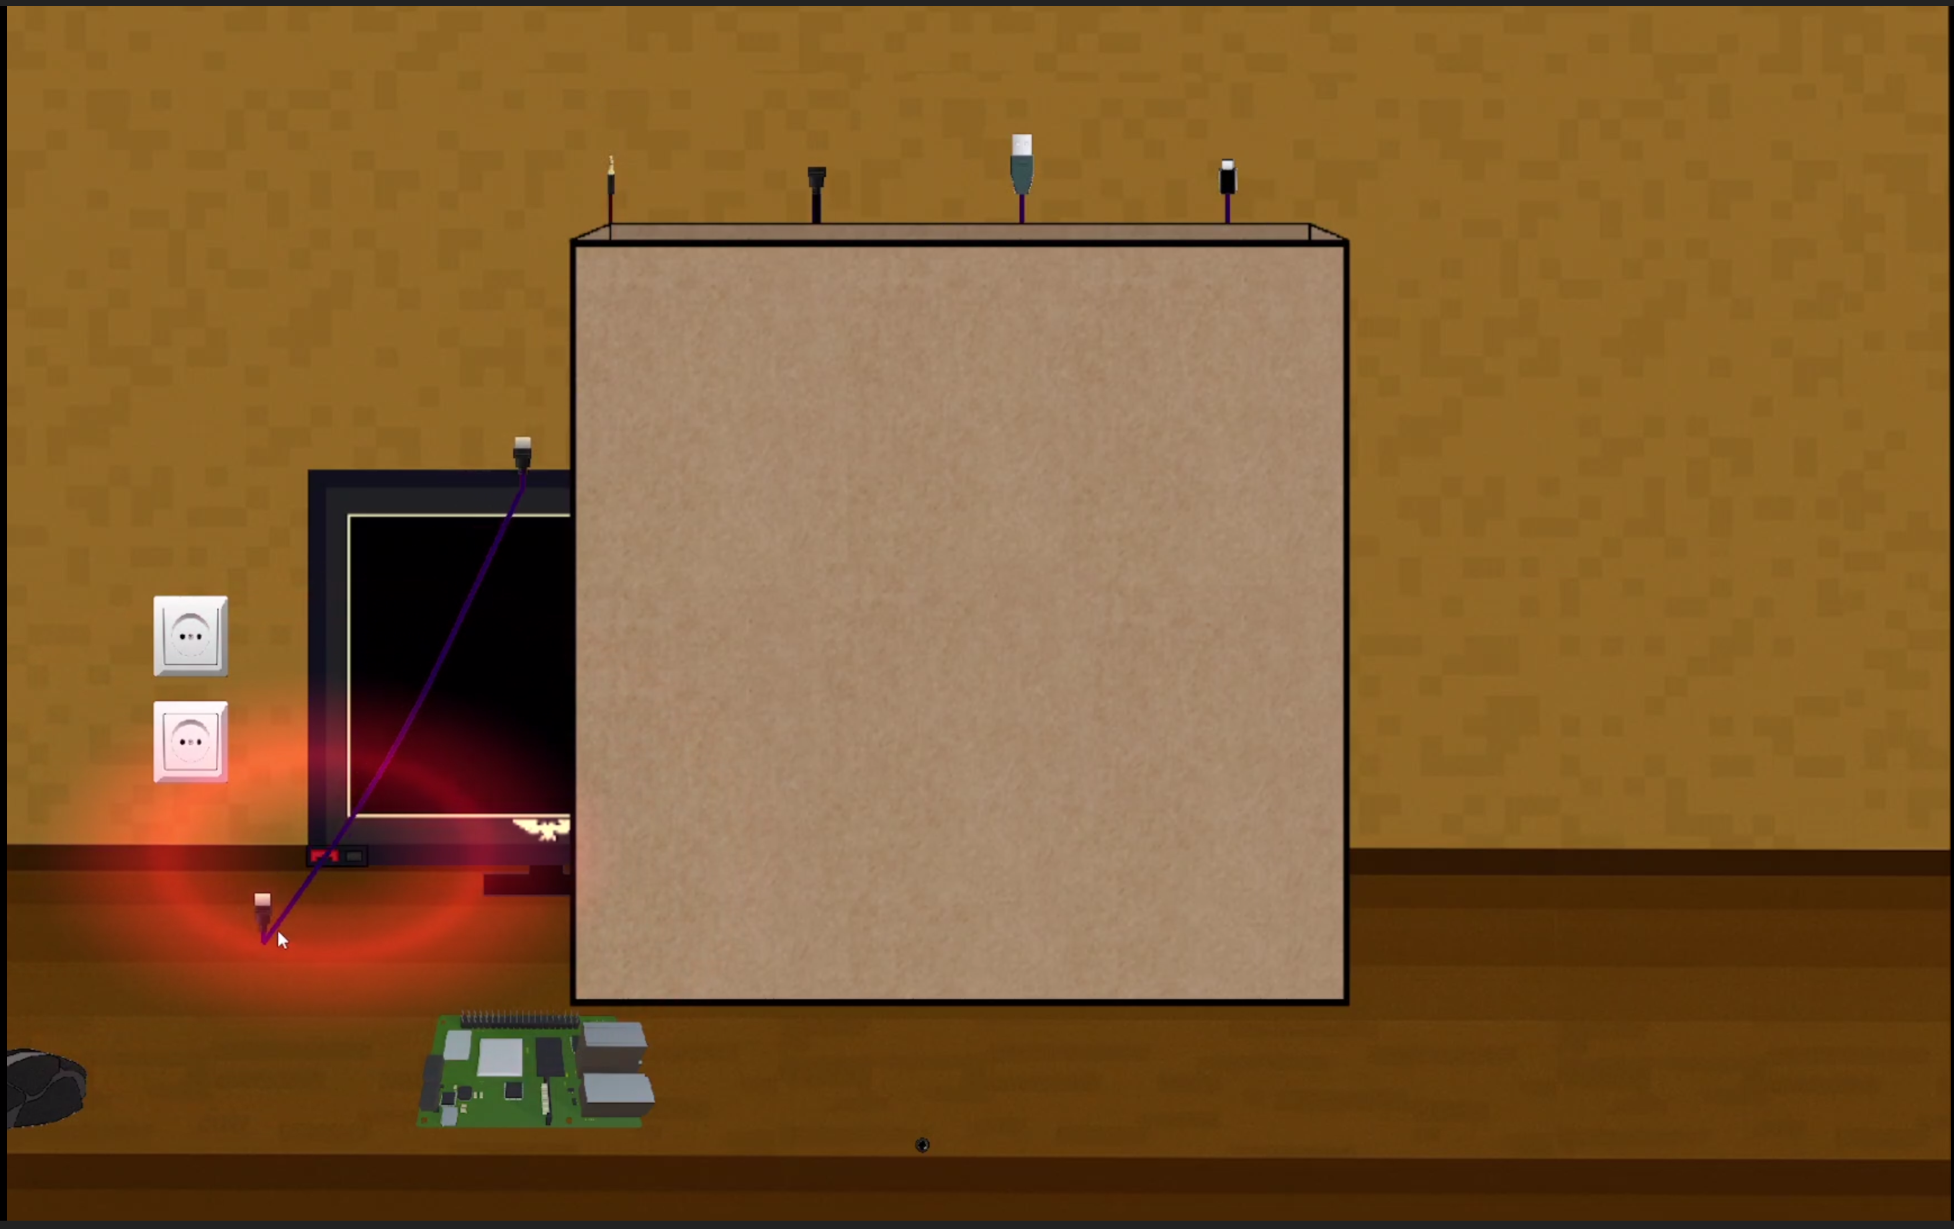
\includegraphics[width=0.7\linewidth]{assets/game1.png}
        \caption{Игровая сцена}
        \label{fig:gamescene}
    \end{figure}
    \item Механика перетаскивания и поворота, игрок может:
    \begin{itemize}
        \item Выбрать устройство из коробки левой кнопкой мыши,
        \item Перемещать его по экрану,
        \item Повернуть с помощью клавиши <<R>> (до 4 положений),
        \item Отпустить устройство в области порта.
    \end{itemize}
    \item Проверка соединения: при отпускании устройства система проверяет:
    \begin{itemize}
        \item Пересечение хитбокса устройства с хитбоксом порта,
        \item Соответствие типов (например, «монитор» "--- <<HDMI>>),
        \item Уникальность подключения (устройство не может быть подключено дважды).
    \end{itemize}
    \begin{figure}[ht]
        \centering
        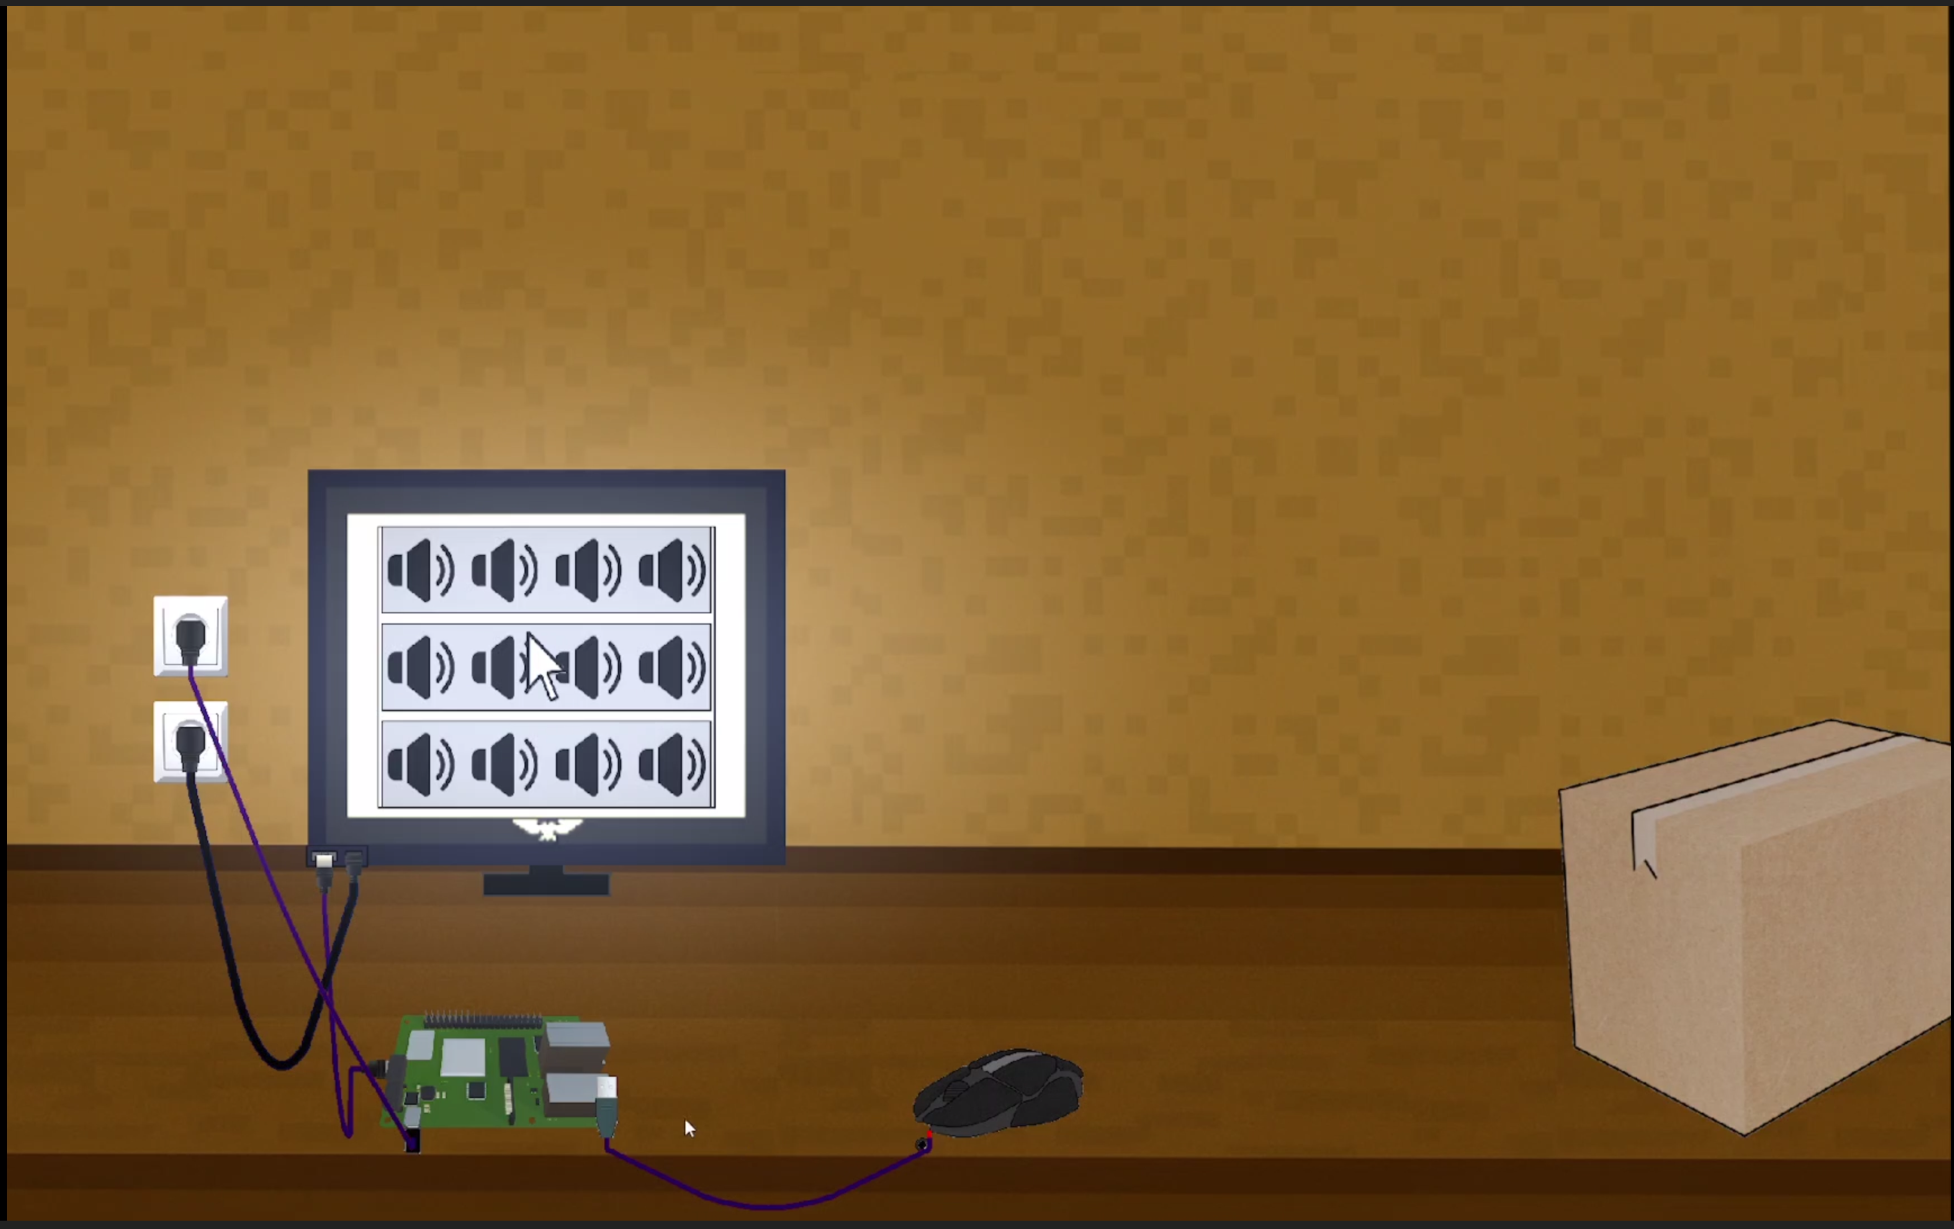
\includegraphics[width=0.7\linewidth]{assets/game2.png}
        \caption{Компьютер подключен верно}
        \label{fig:computerIsOn}
    \end{figure}
    При успешном соединении:
    \begin{itemize}
        \item Устройство <<фиксируется>> на порту,
        \item Проигрывается звуковой фидбек,
        \item Активируется визуальный эффект (например, монитор включается).
    \end{itemize}
    При ошибке "--- отображается подсказка, объект возвращается в коробку.
    \item Инспекция платы. В любой момент игрок может увеличить изображение Raspberry Pi (режим <<осмотр>>), чтобы изучить расположение и назначение портов. Это реализует обучающую функцию: пользователь не просто играет, а изучает реальное устройство.
    \item Завершение уровня. Уровень завершается, когда все обязательные устройства подключены корректно. Корректное подключение устройств указано на рисунке ~\ref{fig:computerIsOn}
\end{enumerate}
Игра не просто имитирует процесс подключения "--- она моделирует типичные сценарии первого знакомства с Raspberry Pi. Особенно важна реализация GPIO (General Purpose Input/Output): даже в упрощённом виде она знакомит пользователя с понятием цифровых/аналоговых пинов, питания (5V/GND) и базовой электроникой.
Планировалось также реализовать мини-приложения внутри <<рабочего стола>> Raspberry Pi (например, терминал, бенчмарк CPU), но из"=за временных ограничений этот функционал был отложен на будущее.